This step is very similar to step 4, however, we can observe the customer features.
Therefore, we can set different price levels for every type of customer.
To leverage this information, every two weeks a context context-generation algorithm is executed.
The algorithm uses a feature tree to select the learner, and it is built using a greedy splitting technique.

\subsection{How to build the feature tree}
Starting from the root node, for each feature the algorithm computes the expected reward without splitting, so by training only a single learner and with splitting on the features, therefore, by training two learners on two partitions of the data.
If the expected reward is larger in the latter case, the node is split in the two cases and the process continues recursively on every new node.
The splitting condition is the following:
\begin{equation}
    p_l\mu_l + p_r \mu_r \geq \mu,
\end{equation}
where \(p_l\) and \(p_r\) are the probability weights and (\mi\), \(\mi_l\) and \(\mi_r\) are the expected reward.

\subsection{Results}
\subsubsection{UCB}
\begin{figure}[ht]
    \begin{center}
    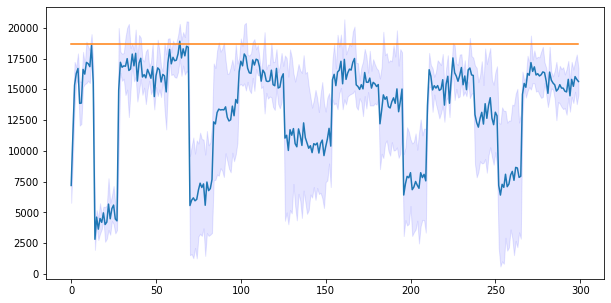
\includegraphics[width=0.6\textwidth]{img/ucb7.png}
    \caption{UCB Reward}
    \label{fig:reward7}
    \end{center}
\end{figure}
\begin{multicols}{2}
    \begin{figure}[H]
        \begin{center}
        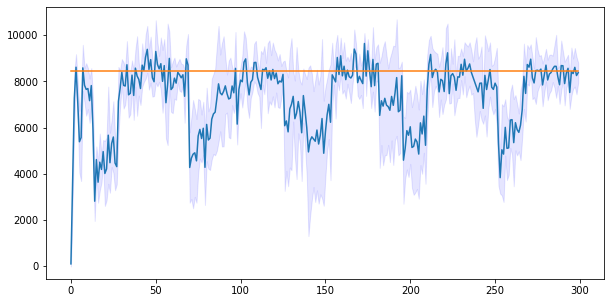
\includegraphics[width=0.5\textwidth]{img/ucb7_1.png}
        \caption{UCB Reward customer 1}
        \label{fig:reward71}
        \end{center}
    \end{figure}
    \columnbreak
    \begin{figure}[H]
        \begin{center}
        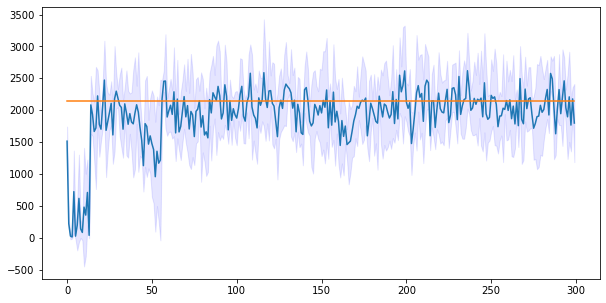
\includegraphics[width=0.5\textwidth]{img/ucb7_2.png}
        \caption{UCB Reward customer 2}
        \label{fig:reward72}
        \end{center}
    \end{figure}
\end{multicols}
\begin{multicols}{2}
    \begin{figure}[H]
        \begin{center}
        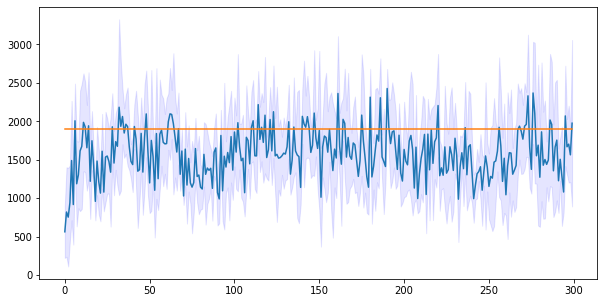
\includegraphics[width=0.5\textwidth]{img/ucb7_3.png}
        \caption{UCB Reward customer 3}
        \label{fig:reward73}
        \end{center}
    \end{figure}
    \columnbreak
    \begin{figure}[H]
        \begin{center}
        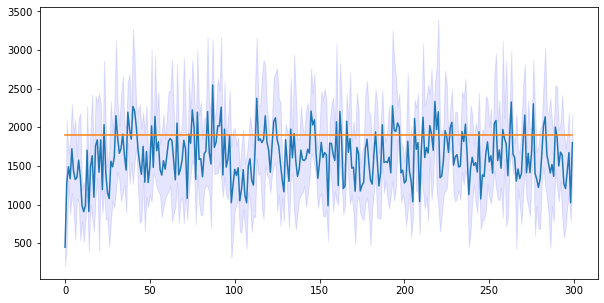
\includegraphics[width=0.5\textwidth]{img/ucb7_4.png}
        \caption{UCB Reward customer 4}
        \label{fig:reward74}
        \end{center}
    \end{figure}
\end{multicols}

\begin{multicols}{2}
    \begin{figure}[H]
        \begin{center}
        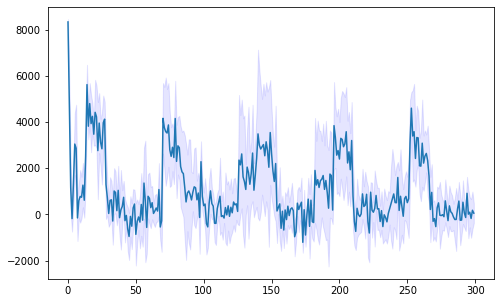
\includegraphics[width=0.5\textwidth]{img/ucb7_1regret.png}
        \caption{UCB Regret customer 1}
        \label{fig:regret71}
        \end{center}
    \end{figure}
    \columnbreak
    \begin{figure}[H]
        \begin{center}
        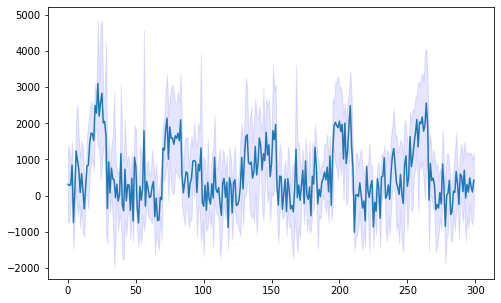
\includegraphics[width=0.5\textwidth]{img/ucb7_2regret.png}
        \caption{UCB Regret customer 2}
        \label{fig:regret72}
        \end{center}
    \end{figure}
\end{multicols}
\begin{multicols}{2}
    \begin{figure}[H]
        \begin{center}
        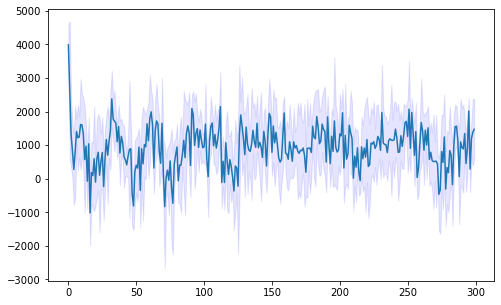
\includegraphics[width=0.5\textwidth]{img/ucb7_3regret.png}
        \caption{UCB Regret customer 3}
        \label{fig:regret73}
        \end{center}
    \end{figure}
    \columnbreak
    \begin{figure}[H]
        \begin{center}
        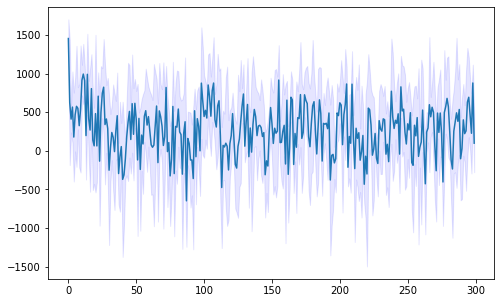
\includegraphics[width=0.5\textwidth]{img/ucb7_4regret.png}
        \caption{UCB Regret customer 4}
        \label{fig:regret74}
        \end{center}
    \end{figure}
\end{multicols}

\begin{multicols}{2}
    \begin{figure}[H]
        \begin{center}
        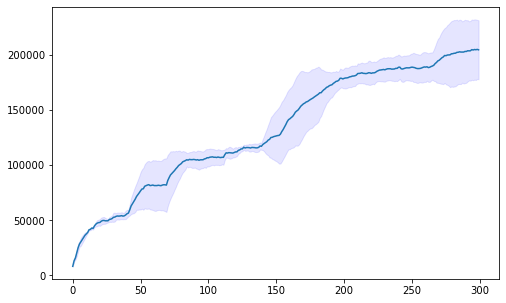
\includegraphics[width=0.5\textwidth]{img/ucb7_1cum_reg.png}
        \caption{UCB Cumulative regret customer 1}
        \label{fig:cum_reg71}
        \end{center}
    \end{figure}
    \columnbreak
    \begin{figure}[H]
        \begin{center}
        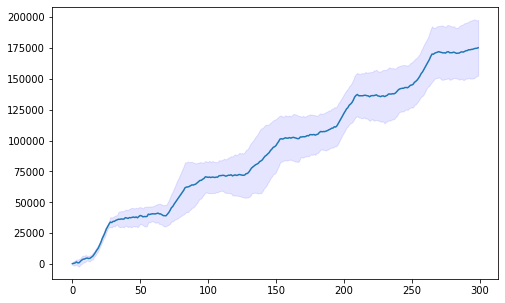
\includegraphics[width=0.5\textwidth]{img/ucb7_2cum_reg.png}
        \caption{UCB Cumulative regret customer 2}
        \label{fig:cum_reg72}
        \end{center}
    \end{figure}
\end{multicols}
\begin{multicols}{2}
    \begin{figure}[H]
        \begin{center}
        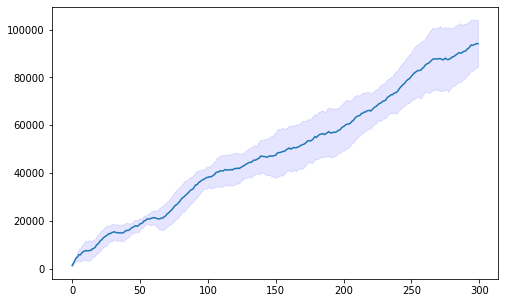
\includegraphics[width=0.5\textwidth]{img/ucb7_3cum_reg.png}
        \caption{UCB Cumulative regret customer 3}
        \label{fig:cum_reg73}
        \end{center}
    \end{figure}
    \columnbreak
    \begin{figure}[H]
        \begin{center}
        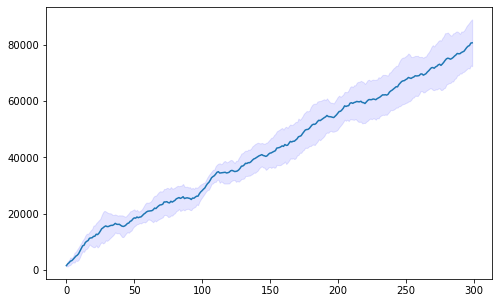
\includegraphics[width=0.5\textwidth]{img/ucb7_4cum_reg.png}
        \caption{UCB Cumulative regret customer 4}
        \label{fig:cum_reg74}
        \end{center}
    \end{figure}
\end{multicols}

\subsubsection{TS}
